\documentclass[]{book}

\usepackage{import}
\usepackage{preamble}
\usepackage{tikz}

\begin{document}

\noindent BECA / Huson / 11.1 IB Math SL \hspace{2in} Name:\\*
30 October 2017
\begin{center}
{\Large Do Now: Exponents and radicals}\\
\textit{Do these problems without a calculator. Use algebra properties to simplify each expression.}
\end{center}

%\vspace{0.2 cm}

\begin{enumerate}

\subsection*{Exponent rules}

\item $\displaystyle 4a^{-2} \times \frac{1}{2}a^4 b^3$\\[10pt]
\item $\displaystyle \frac{5}{2} (x y^2)^2 \times \frac{1}{10}(x^3y)$\\[10pt]
\item $a^3 b \div a^{-4}$\\[10pt]
\item $(-a^3)^3$\\[10pt]

\subsection*{Fractional and negative exponents}

\item $\displaystyle  81^\frac{1}{4}$\\[10pt]
\item $\displaystyle  8^\frac{2}{3}$\\[10pt]
\item $\displaystyle  (0.01)^{-\frac{1}{2}}$\\[10pt]

\subsection*{Radicals and exponents}
Simplify, leaving no negative or fractional exponents.

\item $\sqrt{y^2}$\\[10pt]
\item $\displaystyle  \frac{x \sqrt{25x}}{x^{2}}$\\[10pt]
\item $\displaystyle  \sqrt[4]{\frac{x y^{12}}{z^{4}}}$\\[10pt]




\newpage 

\item Let $\displaystyle f(x) = 2^x$, for $-4 \leq x \leq 4$.
\begin{enumerate}
\item On the  grid below, graph $f$.
\item Write down the value of $f(0)$.
\item Using the graph, solve for $f(x)= \frac{1}{4}$.
\item What is the value of $f^{-1}(4)$?
\end{enumerate}



\begin{figure}[!htbp]
\begin{center}
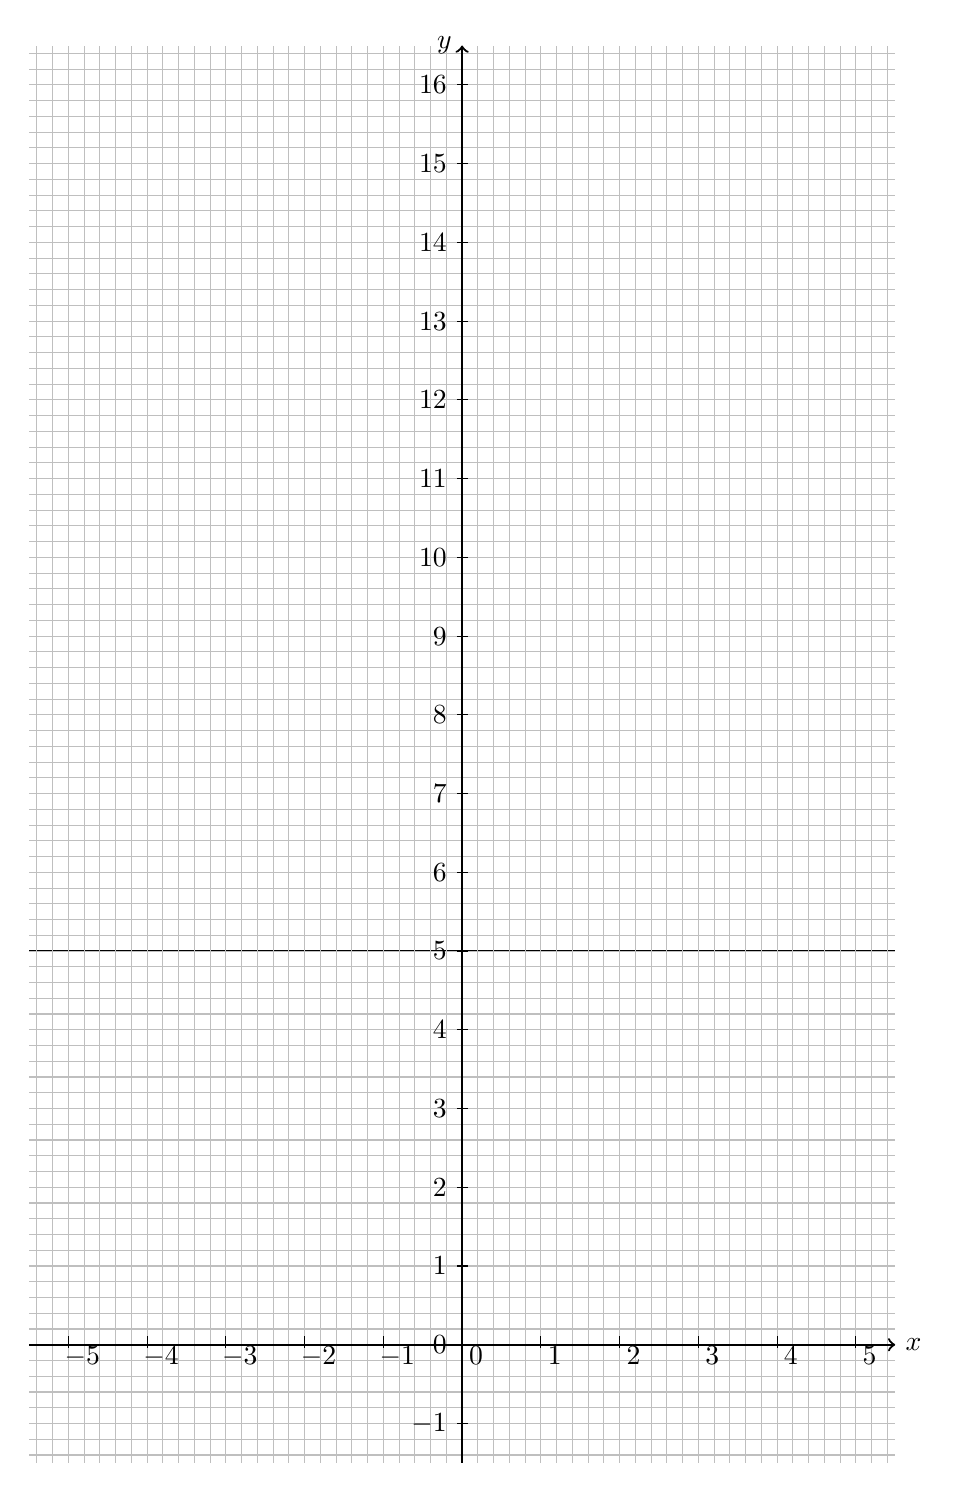
\begin{tikzpicture}

%grid
\draw [color=black,, xstep=1.0cm,ystep=1.0cm] (-5.5,-1.5) grid (5.5,16.5);
\draw [color=lightgray,, xstep=0.2cm,ystep=0.2cm] (-5.5,-1.5) grid (5.5,16.5);

\foreach \x in {-5, -4, -3, -2, -1, 0,1,2,3,4,5}
\draw[shift={(\x,0)},color=black] (0pt,-1pt) -- (0pt,3pt) node[below]  {$\quad \x$};

\foreach \y in {-1,0,1,2,3,4,5, 6, 7, 8, 9, 10, 11, 12, 13, 14, 15, 16}
\draw[shift={(0,\y)},color=black] (2pt,0pt) -- (-2pt,0pt) node[left]  {$\y$};

\draw [thick, ->] (-5.5,0) -- (+5.5,0) node [right] {$x$};
\draw [thick, ->] (0,-1.5) -- (0,16.5) node [left] {$y$};

\end{tikzpicture}
\end{center}
\end{figure}

\end{enumerate}

\end{document}